\documentclass[a4paper,12pt]{report}


%
% Bunch of useful packages
%
\usepackage{etex}
\usepackage[utf8]{inputenc}
\usepackage{algorithmic}
\usepackage{algorithm}
\usepackage{pst-plot}
\usepackage{graphicx}
\usepackage{graphics}
\usepackage{caption}
\usepackage{subcaption}
\usepackage{floatflt}
\usepackage{wrapfig}
\usepackage{endnotes}
\usepackage{amsfonts}
\usepackage{amsmath}
\usepackage{amsthm}
\usepackage{amssymb}
\usepackage{verbatim}
\usepackage{hyperref}
\usepackage{multirow}
\usepackage{endnotes}
\usepackage{pdflscape}
\usepackage{multicol}
\usepackage{tikz}
\usetikzlibrary{arrows}
\usepackage{wrapfig}
\usepackage{hyperref}
\usepackage{array}
\usepackage{rotating}
\usepackage{enumitem}
\usepackage{setspace}
\usepackage{enumitem}

\usepackage[font={small, sl}]{caption}

%
% Listings
%
\usepackage{color}
\usepackage{xcolor}
\usepackage{listings}
\lstset{
	basicstyle=\scriptsize\ttfamily,
	numbers=left,
	numberstyle=\tiny,
	numbersep=5pt,
	tabsize=2,
	extendedchars=true,
	breaklines=true,
	keywordstyle=\color{red},
	frame=b,         
	stringstyle=\color{white}\ttfamily,
	showspaces=false,
	showtabs=false,
	xleftmargin=17pt,
	framexleftmargin=17pt,
	framexrightmargin=5pt,
	framexbottommargin=4pt,
	showstringspaces=false
}
\usepackage{caption}
\DeclareCaptionFont{white}{\color{white}}
\DeclareCaptionFormat{listing}{\colorbox{gray}{\parbox{\textwidth}{#1#2#3}}}
\captionsetup[lstlisting]{format=listing,labelfont=white,textfont=white}

%
% Chapter titles
%
\usepackage{titlesec}
\titleformat{\chapter}[hang] 
{\normalfont\huge\bfseries}{\thechapter}{1em}{} 

%
% Theorems and Definitions
%
\theoremstyle{definition}
\newtheorem{definition}{Definition}[chapter]

%
% Margins of all kinds
%
\hypersetup{pdfborder={0 0 0 0}}
\setlength\parindent{0mm}
\setlength\parskip{3mm}

\newenvironment{pitemize}{
\vspace{-5mm}
\begin{itemize}
 	\setlength{\itemsep}{1pt}
	\setlength{\parskip}{0pt}
 	\setlength{\parsep}{0pt}
}{
	\end{itemize}
	\vspace{-8mm}
}


%%%%%%%%%%%%%%%%%%%%%%%%%%%%%%
%% Width of A4 is 8.27in (210mm) We have an inside margin of 1.5 in and outside margin of 1in
%% This leaves 5.77in for text width
\oddsidemargin=0.5in
\evensidemargin=0.0in
\textwidth=5.77in
\headheight=0.0in
\topmargin=0.0in
\textheight=9.0in
%%%%%%%%%%%%%%%%%%%%%%%%%%%%%%


\newenvironment{sitemize}
{\vspace{-2mm}\begin{list}{\textbullet}{%
    \setlength{\itemsep}{0pt}%
    \setlength{\parsep}{0pt}%
    \setlength{\topsep}{0pt}%
    \setlength{\parskip}{0pt} %
    \setlength{\labelwidth}{0pt}%
    \setlength{\labelsep}{0.05in} %
    \setlength{\leftmargin}{5pt} %
    \renewcommand{\labelitemi}{\textbullet}}}
  {\vspace{-2mm}\end{list}}

\newenvironment{mitemize}
{\begin{list}{\textbullet}{%
    \setlength{\itemsep}{0pt}%
    \setlength{\parsep}{0pt}%
    \setlength{\topsep}{2mm}%
    \setlength{\parskip}{0pt} %
    \setlength{\labelwidth}{0pt}%
    \setlength{\labelsep}{0.05in} %
    \setlength{\leftmargin}{8.5mm} %
    \renewcommand{\labelitemi}{\textbullet}}}
  {\end{list}}


\newcommand\epigraph[3]{
\vspace{1em}\hfill{}\begin{minipage}{#1}{\begin{spacing}{0.9}
\small\noindent\textit{#2}\end{spacing}
\vspace{1em}
\hfill{}{#3}}\vspace{2em}
\end{minipage}}


%
% Title
%
% TODO title would better be a bit shorter. Other possibilities:
% Biologically realistic single neuron model performs unsupervised learning

\begin{document}
\begin{center}
	{\Large
	University of Tartu\\
	Faculty of Mathematics and Computer Science\\
	Institute of Computer Science\\
	Computer Science\\}
	
	\vspace{2.5cm}
	
	{\LARGE Taivo Pungas}\\
	\vspace{0.5cm}
	\begin{spacing}{2}{\Huge\bf \ \ \ Unsupervised learning algorithms implemented by a biologically realistic neuron model}\end{spacing}
	\vspace{0.5cm}
	{\LARGE Bachelor's thesis (9 ECTS)}
\end{center}
\vspace{3cm}
\hspace{7.2cm}{\Large Supervisors: Dr. Raul Vicente\\}
\vspace{-0.5cm}

\hspace{10.4cm}{\Large Dr. Jaan Aru \\}

\ \\
\ \\
Author: .................................................. "......." May 2015\\
Supervisor: ............................................. "......." May 2015\\
\ \\
Approved for defense\\
Professor: ............................................... "......." May 2015\\
\ \\
\begin{center}
	{\Large Tartu 2015}
\end{center}
\thispagestyle{empty}
\pagebreak


%%%
% Abstract
%%%


{\textbf
{\Large Title of thesis in English}}

\textbf{Abstract:}

Lorem ipsum dolor sit amet, consectetur adipiscing elit. Etiam a ultricies sem, vel gravida dolor. Vestibulum lacinia nulla nec massa mollis eleifend. Etiam scelerisque erat in ligula dapibus, et eleifend enim vulputate. Integer quis lobortis neque, eget efficitur felis. Vestibulum vel consequat quam. Praesent volutpat eget massa rutrum fringilla. Maecenas fringilla turpis ut dignissim luctus. Nunc lectus metus, dapibus eu enim ut, rhoncus blandit ligula. Praesent gravida ullamcorper est id pharetra. Mauris tempus ornare sollicitudin. Sed feugiat nec turpis mattis sollicitudin. Aliquam non orci sit amet lorem rutrum euismod et non orci. Aliquam egestas aliquam blandit. Cras quis convallis neque. Integer fringilla pharetra condimentum. Fusce erat eros, pulvinar sit amet orci in, consectetur accumsan eros.

\textbf{Keywords:} taivo, raul, jaan, model, neuro, stuff

\vspace{1.5cm}



{\textbf
{\Large Töö eestikeelne pealkiri}}

\textbf{Lühikokkuvõte:}

Lorem ipsum dolor sit amet, consectetur adipiscing elit. Etiam a ultricies sem, vel gravida dolor. Vestibulum lacinia nulla nec massa mollis eleifend. Etiam scelerisque erat in ligula dapibus, et eleifend enim vulputate. Integer quis lobortis neque, eget efficitur felis. Vestibulum vel consequat quam. Praesent volutpat eget massa rutrum fringilla. Maecenas fringilla turpis ut dignissim luctus. Nunc lectus metus, dapibus eu enim ut, rhoncus blandit ligula. Praesent gravida ullamcorper est id pharetra. Mauris tempus ornare sollicitudin. Sed feugiat nec turpis mattis sollicitudin. Aliquam non orci sit amet lorem rutrum euismod et non orci. Aliquam egestas aliquam blandit. Cras quis convallis neque. Integer fringilla pharetra condimentum. Fusce erat eros, pulvinar sit amet orci in, consectetur accumsan eros.

\textbf{Võtmesõnad:} taivo, raul, jaan, mudel, neuro, värk


\
\thispagestyle{empty}
\pagebreak

\tableofcontents
\newpage


% % % %
% Chapter: Introduction
% % % %

\chapter*{Introduction}
\addcontentsline{toc}{chapter}{Introduction}

% somehow maybe tie in x-risk and AGI?

Your brain is a complex organ capable of very sophisticated thought. Even though the chess-playing supercomputer Deep Blue won the reigning world champion Garry Kasparov, Kasparov was also able to do anything human beings do every day, whereas the computer could only play chess. The human brain is remarkable not for its ability to do one particular thing very well, be it playing chess, reading an article in Nature, preparing a six-course meal, or slam dunking in a basketball game. It is remarkable for being able to do all of those things, and much more.

However, gaining understanding of the brain's information processing mechanisms remains one of the major scientific challenges today. A key aspect of the brain is \emph{neural plasticity}, its ability to change itself over time as new knowledge and experience are accumulated and processed. To understand the dynamics of these changes, computational models are explored to understand how well they explain the brain's behaviour as observed in experiments in neuroscience, and on a more abstract level, how well the models learn to perform well in a variety of tasks.

Artificial systems with significant capacity for learning have recently been created using deep convolutional neural networks in tasks ranging from playing video games \cite{mnih2015human} to describing scenes in natural language \cite{karpathy2014deep}. The neuron models used in these systems are very simple, often composing of a scalar product of the inputs and weights, and a thresholding function. However, evidence from brains has shown that each neuron is a much more complex and powerful information processing unit. There is a clear gap between the computational properties of networks of neurons and the biophysical mechanisms of synaptic plasticity at the cellular level. The primary goal of this thesis is to help narrow this gap.

One way to bridge the gap is to show by numerical simulations what behaviour results from basic principles of neuronal biophysics.

This work explores the behaviour of one particular previously published (with a Nobel-winning physicist among the authors) biophysically realistic neuron model, which has been shown to produce a range of neural plasticity phenomena. In the thesis, behaviour of the implemented model is first validated against previously published work. Then, its input-output relation is characterised for various kinds of input. As an addition to the model, the effect of probabilistic neurotransmitter release is studied. Finally, two simple tasks are simulated to study the neuron's ability to implement principal component analysis, a well-known unsupervised learning algorithm.

The main goals of the work could be formulated as:
1. implement the neuron model and validate its behaviour (against original papers and what is realistic)
2. explore the behaviour of this model
3. find what effects PR has on behaviour
4. find out whether the neuron can perform a simple PCA task

% % % %
% Chapter: Background
% % % %

\chapter{Background and related work}


\section{Overview of related neuroscience}

% Biology of the human brain
\subsection{Neurobiology of the brain}
The brain, a part of the nervous system, is the central information processing organ in animals. The computational properties of the brain arise from the heavily interconnected networks and sub-networks of specialised cells called \emph{neurons}. It has been approximated \cite{herculano2009human} that the human brain consists of $10^{11}$ neurons with $10^{15}$ inter-neuronal connections called \emph{syn4apses}. This work focuses on modelling one of many different types of neurons - pyramidal neurons.


\subsection{Neurons as computational units}
Every model of a brain that aspires for biophysical reality must include a way to model the behaviour of neurons and synapses. Each neuron can be seen as a small unit performing computation on some inputs and producing corresponding output. There are many computational models of neurons, with the level of detail ranging from complex multi-compartment models to very simple models such as those used in many artificial neural networks (ANNs). 

\begin{figure}[h]
    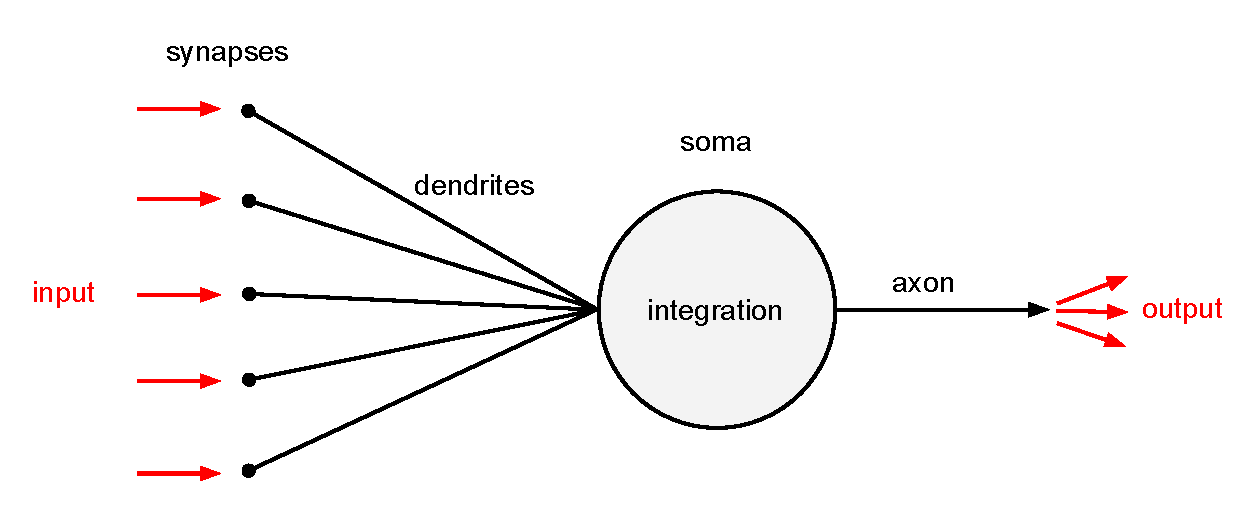
\includegraphics[width=\textwidth]{figures/fig1.pdf}
    \caption{Schematic of a pyramidal neuron.}
    \label{fig:pyramidal}
\end{figure}

Information flow through a neuron follows a path from the inputs to the output, with integration of information in between, as shown in Figure~\ref{fig:pyramidal}. A rough mapping of the corresponding neuron anatomy is also shown.


\subsubsection{Input}

The region of connection between two neurons is called a \emph{synapse}, with information flowing from the axon of the \emph{presynaptic} neuron to a dendrite of the \emph{postsynaptic} neuron. Each time the presynaptic neuron produces significant output, neurotransmitters are released from the presynaptic neuron into the \emph{synaptic cleft}, a small gap between the presynaptic and postsynaptic neurons at the synapse.
Neurotransmitters then bind to receptors on the dendrite of the postsynaptic neuron, causing ion channels to open. This causes ion flow across the membrane, which causes a voltage change at the dendrite of the postsynaptic neuron.

Synapses can be divided into two classes: input arriving at \emph{excitatory} synapses tends to increase the output of the postsynaptic neuron, input to \emph{inhibitory} synapses tends to make it fire less.

\subsubsection{Computation}
A single neuron can be viewed as an integrator of information over time, over different inputs, or both. At each synapse, a neuron has some intrinsic biological components that determine how much this synapse should affect the output of the postsynaptic neuron. \emph{Synaptic weights} are key parameters used in modelling such biological components, and the modification of synaptic weights is the basis of learning in neurons.

After the contribution of input from each synapse is computed, this information must be integrated to produce the output of the neuron. An overview of some of the most common neural models of information integration will be given in Section~\ref{modelsofintegration}.

\subsubsection{Output}

Output of a neuron takes the form of \emph{action potentials} or \emph{spikes}, rapid increases in membrane voltage followed by a return to the equilibrium voltage. Information about action potentials is conducted from a neuron to the dendrites of other neurons using the axon. Axons are usually not part of single neuron models as the output of the modelled neuron is studied in and of itself, so needs not be relayed to other neurons.

\section{Prior work}
%TODO Suggestions from Elena: more detail (obv), examples of published models, what I do differently, why I chose this particular model. Add references.


There are many computational models of neurons, with the level of detail ranging from compartmental to very simple models of a neuron such as those used in ANNs. Using these models, it is possible to simulate neurons in a computer and investigate the models' behaviour in a very controlled and detailed way. As opposed to real experiments that are hindered by many difficulties, using a simulation approach allows detailed investigation and control of input and all parameters.

Two aspects of neurons can be modelled and used in different combinations: the mechanism for translating input signals into output (information integration) and the mechanism for updating synaptic weights (synaptic plasticity).


\subsection{Models of neural information integration}
\label{modelsofintegration}

Some of the best known models, from least to most detailed, are the McCulloch-Pitts \cite{mcculloch1943logical}, integrate-and-fire (IF), and Hodgkin-Huxley \cite{hodgkin1952quantitative} models. In the MP model which is widely utilised in ANNs, a weighted sum of inputs is calculated, to which a sigmoid function is applied to produce the output of the neuron. In the IF and HH models the neuron is modelled as an electric circuit, and then corresponding differential equations are used to calculate the output of the neuron.

%\subsection{Models of synaptic plasticity TODO}

%Different kinds of possible learning rules. Simple ones such as Hebb's rule, Oja's rule, BCM theory. What properties these rules have been shown to have (what behaviours they produce -- PCA etc). Finding learning rules by minimising Fisher information, other information-theoretic measures, or some other objective function \cite{echeveste2014generating}.

%The perceptron \cite{rosenblatt1958perceptron} that works as a simple linear classifier was one of the earliest proposed computational models of the neuron. Since then, numerous models have been proposed. An important characteristic of a neuron model is its mechanism of learning, However, few models explicitly model the biochemistry and physiology leading to synaptic plasticity.


\subsection{Single neuron models in unsupervised learning tasks}

Several single neuron models have been shown to be capable of unsupervised learning: simple artificial neurons can do PCA when trained according to the Oja rule, the tempotron model \cite{gutig2006tempotron} is able to learn spike timing-based patterns, the SKAN model \cite{afshar2014racing} is capable of unsupervised classification of patterns. However, none of the aforementioned models are based on biophysical principles, and no other biophysical models have been shown to do unsupervised learning on the single neuron level.

%Yeung 2004 showed selectivity. But seems that most work about unsupervised learning focuses on networks, not biophysical single neurons.




% % % %
% Chapter: Methods
% % % %
\chapter{Methods}

\section{Input generation}
Rather than simulating presynaptic neurons, inputs to the model are simulated as $N$ spike trains, one for each excitatory synapse, with a given mean firing rate $r$ specified independently for each synapse. Due to the way information is represented in computers, time is discretised into time-steps of length $dt$ regardless of the continuous nature of the biophysical processes. Each spike train one binary number per time-step: 1 if a spike occurred and 0 otherwise. The spike trains are produced in a homogeneous Poissonian process, i.e. the occurrence of a spike is independent of the time since the last spike, and the average rate of spikes remains constant over time.
Correlation between inputs is achieved by specifying the correlation parameter $0 \leq c \leq 1$, and using code from \cite{macke2009} to generate correlated homogeneous Poissonian spike trains. For $c=1$, all synapses receive identical input; for $c=0$, all synapses receive independently generated spike trains.

In all simulations, inputs to inhibitory synapses are generated as uncorrelated Poissonian spike trains with a mean firing rate of 10Hz.

\begin{figure}[h]
    \includegraphics[width=\textwidth]{figures/methods_sample_input.eps}
    \caption{Sample input to 30 synapses, generated for a 1000ms period with a 0.1ms time-step. In this figure, black bars indicate timesteps at which spiketrains (running horizontally) contain spikes. Synapses 1-10 receive 5Hz uncorrelated input, synapses 11-20 receive 40Hz correlated input with $c=0.8$, synapses 21-30 receive 40Hz uncorrelated input.}
    \label{fig:methods_sample_input}
\end{figure}

\section{Neuron model used in simulations}

The neuron model used in this work follows the model of a single neuron published in \cite{yeung2004synaptic}. An integrate-and-fire model of information integration is used with a calcium-dependent model of synaptic plasticity \cite{shouval2002unified}. No dendritic distance is simulated, i.e. the possibility that some synapses are situated further from the soma is not taken into account. In this section, an overview of the most important aspects of the model will be given. The total number of synapses is 120, with 100 excitatory synapses and 20 inhibitory synapses.
% TODO Appendix letter may change.
% TODO do we use metaplasticity? prolly not because don't want to simulate that long.










\subsection{Integrate-and-fire model}

The postsynaptic neuron is modelled as a Traub-Miles cell, which is a Hodgkin-Huxley-like model for estimating postsynaptic voltage. The equations and parameters from \cite{ermentrout1998fine} are used, with one significant difference in parameters: the basal current $I_0$, which causes spontaneous voltage increase, is set to $0$. Compared to Hodgkin-Huxley, the Traub-Miles model includes a more detailed simulation of Na\textsuperscript{+} and K\textsuperscript{+} currents by modelling the dependence of the gating of abovementioned channels on postsynaptic voltage.

The core of the integrate-and-fire model used in this thesis are five currents affecting postsynaptic voltage: a voltage-increasing current caused by presynaptic spikes at excitatory synapses, a voltage-decreasing current caused by presynaptic spikes at inhibitory synapses, Na\textsuperscript{+} and K\textsuperscript{+} currents not directly affected by presynaptic spiking, and a leak current, which tends to return voltage to the resting potential $V_{rest}=-65\mathrm{mV}$. When postsynaptic voltage $V_{post}$ reaches the threshold $V_{thres}=-55\mathrm{mV}$, a postsynaptic spike is recorded, and $V_{post}$ is set to the spiking voltage $V_{spike}=40\mathrm{mV}$. In the next time-step, $V_{post}$ is returned to the reset potential $V_{reset}=-65\mathrm{mV}$, from where it returns to the baseline voltage.

As an addition to the Traub-Miles model, spike-frequency adaptation is implemented following \cite{yeung2004synaptic}: the resting voltage is decreased by 2mV upon each postsynaptic spike, and decays back to the baseline with a time constant of $100\mathrm{ms}$. This temporarily increases the gap between resting and threshold voltages, requiring more presynaptic input to reach the threshold and thus decreasing firing rate.




\subsection{Model of synapses}

Excitatory and inhibitory synapses are modelled by ion gates controlled by the respective neurotransmitters: glutamate and gamma-aminobutyric acid (GABA). Upon each spike at an excitatory synapse, the opening of glutamate-controlled ion channels at dendrites is simulated, with the degree of opening simulated as a sum of two decaying exponentials peaking at the time of spike. The resulting ion flow tends to drive $V_{post}$ towards the excitatory reversal potential $V_{rev,exc}=0\mathrm{mV}$. Similarly, upon each spike at an inhibitory synapse, the opening of GABA-controlled ion channels is simulated, and the resulting ion flow tends to drive $V_{post}$ towards the inhibitory reversal potential $V_{rev,inh}=-65\mathrm{mV}$. Spikes at excitatory synapses have a larger relative influence on $V_{post}$) due to the higher simulated conductivity (maximum throughput of ions) of glutamate-controlled ion channels.

The effect of presynaptic spikes on the gating of glutamate-controlled and GABA-controlled channels is simulated according to the model from \cite{borgers2008gamma}.

%FIGURE: spatial and temporal summation of EPSP-s, causing a spike (action potential) vs not causing a spike. Also on same timeline, an IPSP. Below, show excitatory and inhibitory spikes as raster plots. I think Julius had a good figure for this.




\subsection{Plasticity}

In addition to components mentioned in the previous section, the extent to which presynaptic spikes influence postsynaptic voltage is modelled by the synaptic weights $\boldsymbol{W}=(W_i)$, with $i$ denoting the number of the synapse. The modification of these weights is the basis of learning in this model: increasing $W_i$ will increase the effect spikes at the $i$-th synapse have on postsynaptic voltage, and vice versa. In this model, only excitatory synapses are plastic, i.e. the weights of inhibitory synapses remain unchanged.

%TODO use Shouval Scholarpedia article for explaining basis of learning (http://www.scholarpedia.org/article/Models_of_synaptic_plasticity#Calcium_dependent_models_of_bidirectional_synaptic_plasticity)
The mechanism for modifying synaptic weights follows the Ca\textsuperscript{2+}-dependent model from \cite{shouval2002unified}, where the aim was "to construct a model based on a minimal number of assumptions". The model detects coincidences of presynaptic and postsynaptic spikes: the weight of synapse $i$ will be increased if the presynaptic spike occurs right before the postsynaptic spike (i.e. there is reason to believe the postsynaptic spike was \emph{caused} by the input), and decreased otherwise. The process of spike-timing-dependent plasticity (STDP) captures this idea that learning should depend on the exact timing on postsynaptic and presynaptic spikes. It was shown in \cite{shouval2002unified} that the plasticity model used in this work implements STDP in a way similar to what has been observed in experiments in neuroscience.

The mechanism for detecting coincidences relies on N-methyl-D-aspartic acid (NMDA) receptors. NMDA receptors control gates that can allow calcium ions to flow into the neuron, which in turn causes an increase of the synaptic weight. The extent to which the calcium channels open depend on two factors: concentration of glutamate (the neurotransmitter that also causes voltage increases upon spikes at excitatory synapses) and dendritic voltage caused by a back-propagating action potential (BPAP). The former relays information about presynaptic spikes: if a spike has occurred recently, the level of glutamate at the synapse is at a high level. The latter signifies a postsynaptic spike: when the postsynaptic neuron fires, an increase in voltage is propagated to the dendrites. The influx of calcium is dependent on the exact timing of spikes because both glutamate concentration and BPAP voltage decay in time. The synaptic weights' update depends on the level of intracellular calcium as shown in Equation~\ref{eq:weightupdate}, with shapes of $\Omega$ and $\eta$ shown in Figure~\ref{fig:methods_eta_omega}.

\begin{equation}
\frac{dW_i}{dt} = \eta ([Ca]_i) (\Omega([Ca]_i) - \lambda W_i)
\label{eq:weightupdate}
\end{equation}

This mechanism allows the synaptic weights to increase when there has been a suitably timed pair of presynaptic and postsynaptic spikes. However, \cite{shouval2002unified} show that the same mechanism also accounts for decreasing and stable synaptic weights through the effect of $\Omega$: at medium levels of Ca\textsuperscript{2+}, weights are decreased ($\Omega<0.5$), and at low levels of Ca\textsuperscript{2+}, synaptic weights remain unchanged ($\Omega$ is constant at 0.5). The learning rate $\eta$ also depends on calcium: higher levels of Ca\textsuperscript{2+} elicit larger changes in synaptic weights. $\lambda$, together with the value of $\Omega$ in the range of low calcium, determine the stable point of synaptic weights.

The phenomenon of synaptic weights increasing due to learning is named long-term potentiation (LTP), and similar decreasing is named long-term depression (LTD). LTD and LTP are the methods the neuron uses to assign different synaptic weights based on the input to that synapse.

\begin{figure}[h]
    \includegraphics[width=\textwidth]{figures/methods_eta_omega.eps}
    \caption{This is a caption.}
    \label{fig:methods_eta_omega}
\end{figure}


\subsubsection{Metaplasticity}
\emph{Metaplasticity} refers to plasticity of synaptic plasticity - the dependence of plasticity on the history of the previous activity of the neuron. In the scope of this thesis, it refers to the changing of NMDA receptor (NMDAR) conductance as a function of output voltage, which leads to changes in the calcium influx and therefore changes in the sign and magnitude of changes in synaptic weights. The model of metaplasticity follows that of \cite{yeung2004synaptic}, where the NMDAR conductance $g$ is the same for all synapses and is updated according to the following equation: $$ \frac{dg}{dt}=-(k_- (V-V_{rest})^2 + k_+)g + k_+ g_t $$
Here, $g_t$ shows the total supply of NMDARs available in the internal pool of the neuron. $k_+$ and $k_-$ are kinetic constants describing the speed of insertion and removal of NMDARs into synapses.

Metaplasticity can be disabled in any simulation, resulting in a constant value of $g$.





\section{Implementation details}

The model was implemented and data analysis conducted in MATLAB; source code is attached as an online supplementary to the thesis. The simulations were carried out in part in the High Performance Computing Center of University of Tartu.

For updating values according to the differential equations, the Euler method is used with a 0.1ms time-step length, chosen as the highest value allowing numerical stability. At the start of each simulation, some parameters are initialised to previously found equilibrium values to avoid unstable behaviour. Input is generated in 1-second blocks for ease of implementation, and the release of neurotransmitters caused by each presynaptic spike is assumed to last 1 ms. The computational complexity is linear with respect to the total simulation time; the computation time required for $x$ seconds of simulated neuron time varies between $2x$ and $15x$ seconds on the machines used for simulation and depends on the amount of input to the neuron.

Unless mentioned otherwise, learning speed was increased by a factor of 100 by multiplying the values of learning rate $\eta$ and NMDA receptor kinetic constants $k_+$ and $k_-$ by 100. According to \cite{yeung2004synaptic}, the fixed points of the system do not change upon speeding up the simulations by this factor.











% % % %
% Chapter: Results
% % % %
% Useful link for figures: http://tex.stackexchange.com/questions/37581/latex-figures-side-by-side
\chapter{Results}

\section{Validation of model behaviour}

As a prerequisite to analysing more complex behaviour of the model, it is necessary to make sure the model is implemented correctly. Syntax and other obvious errors aside, the simplest way to do this is to observe the behaviour of the model under some conditions and compare the result with previously published results on the same model in the same conditions. As \cite{shouval2002unified} and \cite{yeung2004synaptic} form the basis of the model, the behaviour of the model implemented in this thesis will be compared to these two sources. Attention will also be paid to keeping parameters and outputs in biophysically realistic ranges.

\subsection{Input-output relationship}
\label{subsec:iocurve}

The input-output curve of a neuron is one of the most important characteristics, showing the output of the neuron to a specified amount of input. The exact scale of the curve is highly dependent on the specific parameters used. In particular, EPSP amplitude has a major effect on this relationship. 
Figure~\ref{fig:valid_iocurve_vs_epsp_grid} shows the curve for 6 different neurons, each with a different EPSP amplitude. It is evident that the relationship is linear for a range of EPSP amplitudes, which is consistent with the findings of \cite{yeung2004synaptic} for simulations with metaplasticity enabled. For low values of EPSP amplitude and input rate, there is no output, indicating subthreshold activity: postsynaptic voltage never reaches the threshold required for producing a spike.

Increasing EPSP amplitude by a factor, the curve remains linear, but output rates are scaled up by a similar factor. This means the plausible EPSP voltage range is not much constrained by considering the shape of the input-output curve, and EPSP voltage can be tuned to scale the output of the neuron according to other considerations. The EPSP amplitude producing the closest curve to that of \cite{yeung2004synaptic} lies between 1.0mV and 2.0mV. However, another crucial consideration here is biophysical reality: for completely unstructured input (noise) at 30Hz, a firing rate of even 40Hz is excessive. For this reason, in further simulations EPSP voltage was set to 3.0mV, a value found to produce good results in other informal parameter sweeps.


\begin{figure}[h]
    \includegraphics[width=\textwidth]{figures/valid_iocurve_vs_epsp_grid.eps}
    \caption{Input-output relationship of the neuron for different values of EPSP amplitude parameter (shown above each plot). Each data point in a plot is one experiment, in which input to the neuron consists of uncorrelated spike trains with mean input rate per synapse shown on the x-axis. Due to plasticity and metaplasticity, output rate varies until a fixed point is reached; for this reason, output rate is measured over the last 500 seconds in a 10000-second experiment.}
    \label{fig:valid_iocurve_vs_epsp_grid}
\end{figure}




\subsection{Spike timing-dependent plasticity}

A spike-timing-dependent plasticity curve is important aspect of neuron models: it shows how the neuron determines the sign and magnitude of  synaptic weight updates in response to the relative timing of pre- and postsynaptic spikes. In the model used here, two parameters significantly affect STDP curve shape: BPAP amplitude and the amount of glutamate released on the presynaptic side upon each spike. The shape of STDP curve using parameters from \cite{yeung2004synaptic} is given in Figure~\ref{fig:valid_stdp}A. For comparison, Figure~\ref{fig:valid_stdp}B shows the same figure for a higher BPAP amplitude 100mV, which is the value used in \cite{shouval2002unified}.

Both curves are qualitatively similar to \cite{shouval2002unified} with two regions of LTD induction--one at negative values of $\Delta t$ and another in the region of $\Delta t > 100\mathrm{ms}$--and a single region of potentiation in between. However, for BPAP amplitude 100mV, the curve is smoother and weight differences larger, indicating that BPAP amplitude can be used for tuning STDP curve as necessary. In all following simulations, BPAP amplitude is fixed to 42mV to adhere to parameters published in \cite{yeung2004synaptic}.




\begin{figure}
\centering
\begin{minipage}{.5\textwidth}
  \centering
  \includegraphics[width=1\linewidth]{figures/valid_stdp_bpap42.eps}
\end{minipage}%
\begin{minipage}{.5\textwidth}
  \centering
  \includegraphics[width=1\linewidth]{figures/valid_stdp_bpap100.eps}
\end{minipage}
\caption{\textbf{A.} STDP curve for BPAP amplitude at 42mV. The relative timing of pre- and postsynaptic spikes $\Delta t = t_{post} - t_{pre}$ is plotted on the x-axis, and the weight resulting from a 100-second 1Hz stimulation of pre-post spike-pairs with the respective $\Delta t$ is on the y-axis. The dashed line shows the value to which synaptic weights converge in the absence of postsynaptic spikes.
\textbf{B.} STDP curve for BPAP amplitude at 100mV. Note the change in scale.}
\label{fig:valid_stdp}
\end{figure}




\subsection{Metaplasticity}

The simplest effect of metaplasticity studied by \cite{yeung2004synaptic} was a slow scaling down of weights after an fast potentiation, or scaling up of weights after a fast depression. In both cases, the fast change is induced by regular synaptic plasticity, and the subsequent scaling my metaplasticity. In Figure~\ref{fig:valid_metaplasticity_evolution}, these dynamics are visible: after an initial quick potentiation, weights are slowly scaled down to a value where they remain stable.

The model produces another effect of metaplasticity observerd in \cite{yeung2004synaptic}: increasing the width of the weight distribution and breaking the symmetry of almost-equal weights. After the initial quick increase in weights, the standard deviation of weights increases significantly.

\begin{figure}[h]
    \includegraphics[width=\textwidth]{figures/valid_metaplasticity_evolution.eps}
    \caption{Evolution of synaptic weights in a metaplasticity experiment. For weights of excitatory synapses, both the mean (blue line) and $\pm$1 standard deviation range (grey area) are shown. Input to all synapses was uncorrelated with a mean rate of 20Hz.}
    \label{fig:valid_metaplasticity_evolution}
\end{figure}




\subsection{Selectivity to temporal correlation} % aka temporal code

Temporal correlation between spike trains, i.e. increased probability of coincidence of spikes, indicates underlying structure in the input. Thus, if the neuron is to learn this structure, in the presence of two groups of inputs with only one group correlated, the synapses of correlated inputs should be selectively potentiated. A strong effect of this sort is observed in \cite{yeung2004synaptic}, with weights of the uncorrelated channel going to zero. However, it can be seen in Figure~\ref{fig:selectivity_correlation} that in the model used in this thesis, the selectivity to correlation is weak: the difference in weights of the two channels is existent but small, the group mean weights differing by approximately 20\%. An informal parameter sweep was conducted, but selectivity to correlation did not increase.

\begin{figure}[h]
    \includegraphics[width=\textwidth]{figures/valid_selectivity_correlation.eps}
    \caption{Evolution of synaptic weights over time in a selectivity experiment. Synapses 1-25 receive correlated input ($c=0.8$) at 30Hz, synapses 26-100 receive uncorrelated input at 30Hz. The values of synaptic weights were sampled every 100ms.}
    \label{fig:selectivity_correlation}
\end{figure}









\section{Learning patterns of input rate}

As shown in Section~\ref{subsec:iocurve}, the neuron's output rate is dependent on its input rate. In this section, I will study the neuron's ability to learn and respond to patterns encoded in the mean firing rates of inputs. First, it will be shown that the neuron distinguishes between learned inputs and noise. Secondly, the neuron will be shown to be linear upon presenting learned input patterns partially. Finally, the effect of pattern width on learning will be studied.

\subsection{Response to learned inputs}
\label{subsec:learnedinputs}
% Experiment 2 and Experiment 6: the neuron learns to fire more for a learned input than for a non-learned input.

% Experiment 2

Before investigating the neuron's ability to learn complex input patterns, it is necessary to ensure the neuron is capable of learning anything at all. In particular, it should be capable of distinguishing between a learned pattern and random noise. To study this, a neuron was trained on Pattern 1 (shown in Figure~\ref{fig:exp2_inputpatterns}) consisting of high-rate (40Hz) input to 25 synapses, and low-rate (10Hz) background input to all other synapses, both the pattern and background uncorrelated.

\begin{figure}[h]
    \centering
    \includegraphics[width=\textwidth]{figures/exp2_inputpatterns.eps}
    \caption{Caption lalala.}
    \label{fig:exp2_inputpatterns}
\end{figure}

After training, plasticity and metaplasticity were disabled by fixing the weights, and two tests were run. In Test 1, the neuron received exactly the same input as in training. As control, in Test 2, the 25-synapse high-rate pattern was shown to a different, non-overlapping set of synapses, with all other synapses receiving background input at 10Hz, so the total amount of spikes received by the neuron in both tests remained constant. The resulting output rate for Test 1 was 64Hz and for Test 2 44Hz, suggesting that the neuron fired more when it was presented with the learned input (compared to non-learned input).

Training: I train the neuron on a high-rate 'bump': 40Hz to synapses 1...25 and 10Hz to all others.
Test: two cases.
Case 1: input is exactly the same as training input: 40Hz bump at synapses 1:25.
Case 2: input is changed only by changing the location of the bump by moving it to synapses 76:100.

I anticipated that in Case 2 the neuron fires less (because it gets less input to the synapses that were potentiated due to learning the 40Hz input), and the experiment confirmed this: Case 1 produced 64Hz output, Case 2 produced 44Hz output (the difference remains at ~20Hz in all runs).
This result may seem trivial but I did this to show that the neuron does not fire a lot any time it sees a bump anywhere, but responds most only if the bump was the pattern that it was shown during training.

% Experiment 6

Training: 40Hz input to 25 synapses, 10Hz to others.
Testing: pattern changes every 1000ms. For 1000ms, the pattern is the same as training pattern; for the next 1000ms the neuron gets flat input (same total rate); then training pattern etc.

To find the instantaneous firing rate, I count spikes using a sliding time window of varying size.
On the bottom plot, the red dashed lines show the mean output rate for time periods with patterned input (top line => higher rate) and with flat input (bottom line => lower rate).

The result is as expected: the neuron fires more when it sees the learned pattern, and switches to a lower rate when it gets noise.
I would probably place this near Experiment 2 since the points are pretty similar; what Experiment 6 adds is time-dynamics and a nice graph showing that the neuron indeed switches between two modes of firing if it sees two modes of input.

Instantaneous rate at time t is the count of postsynaptic spikes in the time window [t-500ms, t+500ms].

COMMENT on high firing rates: this is something I did contemplate myself. I think the main culprits are the exact values of two parameters: EPSP voltage and the stable point of weights. Drawing a plot that shows an input-output curve for a bunch of different EPSP values should take no more than 10 minutes (I have all the code), so I'll put this figure along with a description of other likely causes somewhere into Results > Validation. A weak justification is also that Shouval 2004 have high rates too (at least for an untrained neuron - 30Hz uncorrelated input results in 60Hz output).


\begin{figure}[h]
    \includegraphics[width=\textwidth]{figures/exp6_voltageoscillation.eps}
    \caption{Caption lalala.}
    \label{fig:exp6voltageoscillation}
\end{figure}







\clearpage % TODO remove
\subsection{Response to partial presentation of learned inputs}
\label{subsec:partialpatterns}
% Experiment 1 and Experiment 5: the neuron responds linearly to varying input intensity (Exp 1) and proportion of pattern present (Exp 5).

% Experiment 1
Train: I train the neuron on uncorrelated input, with synapses 1...25 getting 40Hz and all others getting 10Hz.

Test: I test the neuron by giving synapses 1...25 inputs ranging from 0Hz to 70Hz (each one a different run) and all other synapses getting such inputs that the total input received by the neuron remains constant in each run. Plotted is the output rate from each run (blue line).

Control (orange line): I trained another neuron (another instance) on uncorrelated input with all synapses getting the same input (but the total input received by the neuron still constant). Results are shown below.

Note that the black dashed line shows the point where all inputs get the same input (17.5Hz). Left of that line, synapses 1...25 get lower input than the others, and vice versa.

Basically, I vary the intensity of a learned input pattern and see what output the neuron produces. I think the result is interesting in that  shows what filter the neuron implements - a linear one. This can be compared with what is done in ANNs where they have rectified linear or sigmoidal filters. It seems to me that the analogy holds very well, and that this result is very useful in the context of building a network of these neurons (as well as general understanding of how the neuron behaves).

It's also interesting that the neuron is linear in the region left of the dashed line as well, i.e. the neuron also linearly determines the absence of input.

% Experiment 5
Training: train a neuron by showing channel 1 (40 synapses) a high input rate of 40Hz, and all others such a rate that total input to neuron is 1750Hz.
Testing: take a subset of the original 40 synapses trained on high input, and show them the same input as before. All others get a lower rate so the total input to neuron is 1750Hz.
Comparison: train a neuron on flat input (with total input rate staying the same at 1750Hz), and test in the same way.

So I train the neuron on some pattern coded in X synapses, and then show the same pattern only partially (less than X synapses).

I think the most interesting result here is that
1. the neuron doesn't do pattern completion (which I anticipated since with learning disabled, the neuron fires more when there is more input) and
2. the neuron responds to removing synapses pretty linearly, similar to its linearity when decreasing the input rate (experiment 1).

Thinking of the result of experiment 1, there is actually also an implication for probabilistic release. Due to the linearity of the neuron, if there is a 50\% probability of release (effective input rate is 50\% of actual rate R), the output rate of the neuron will also be 50\% of the way between baseline and what one would expect for a rate R.
(I think the above is good to mention in the Discussion section of the thesis.)

\begin{figure}
\centering
\begin{minipage}{.5\textwidth}
  \centering
  \includegraphics[width=1\linewidth]{figures/exp1_filter.eps}
  \captionof{figure}{A figure}
  \label{fig:test1}
\end{minipage}%
\begin{minipage}{.5\textwidth}
  \centering
  \includegraphics[width=1\linewidth]{figures/exp5_patterncompletion.eps}
  \captionof{figure}{Another figure}
  \label{fig:test2}
\end{minipage}
\end{figure}







\clearpage % TODO remove
\subsection{Response to patterns with different channel widths}
\label{subsec:patternwidths}
% Experiment 4: the neuron becomes more selective to patterns coded in a particular number of synapses (or a small range).

Training: give a total of 1000Hz input to channel 1 (synapses 1...w), and 750Hz to channel 2 (all other synapses), varying w (the width of channel 1) from 10 to  50.
Testing: give exactly the same input as in training.
Comparison: train the neuron on flat input with the same total rate.

So I vary the width of a pattern channel to find out, what would be the 'optimal' width of a pattern, i.e. the optimal amount of synapses to use to encode a pattern. The resulting line is shown in blue (with +- 1 standard deviation lines), with the comparison in orange.

It turns out that even though the neuron fires most for 20...25-synapse patterns, the neuron is more selective to patterns that are coded in fewer synapses (selectivity here is the difference between the blue and orange line, and the difference is largest for low numbers of synapses).

Using this graph, I would argue that it does make a difference exactly how you create the pattern you're going to use with this model -- and coding a pattern in 10-20 synapses elicits selectivity well, whereas a 40-50 synapse pattern doesn't. This makes sense, since a few very strongly firing inputs seem to convey better information than a large amount of inputs that have only slightly higher rates than background.
The value of this knowledge: it helps inform further experiments by showing what kind of parameters to use.

\begin{figure}[h]
    \centering
    \includegraphics[width=0.5\textwidth]{figures/exp4_synapsecount.eps}
    \caption{Caption lalala.}
    \label{fig:exp4synapsecount}
\end{figure}






\clearpage % TODO remove
\section{Probability of release} % or [Investigating] the effect of probability of release

% Experiment 8
Testing what the input-output curve looks like for different values of PR (the input will have correlation of c=0.8 because otherwise the effect of PR is to only change the rate of input).
Disabled resting voltage dynamics and reduced the weights. Also changed EPSP? (Look at the figure file name to find out.)

% Experiment 7
* Fix syn. weights so that 5 weights are at 1.0 and all others at 0.05.
* Select input rate r.
* Select probability of release parameter p.
* Generate input by starting with perfectly correlated input with a rate of r/p, and randomly remove each spike with probability 1-p (i.e. probability of keeping it is p. The rate r is divided by p so the effective input to the neuron is always the same.
* Measure output rate of the neuron as a function of probability of release p; do this 10 times for each value of p and find the mean and stdev of output rates in these 10 experiments.

The hypothesis is that there exists an optimal value of p, for which some measure of informational goodness is highest, and for any other p (higher or lower), this measure will decrease.
The two measures I'm looking at are, as mentioned, the mean output rate and the variance in output rates. High variance in the output can be good because the range of outputs available to the neuron is wider.

The (faulty) results I got earlier today were interesting in that sense: there was a peak in both mean and variance of output rate at p=0.3 to p=0.5 The correct results are attached; the filename gives away the input rate used. The correct results are pretty linear compared to the faulty ones; this difference is explained by the fact that right now I am operating in the linear range, whereas for the faulty results I operated in a highly non-linear regime of the neuron.

The conclusion that I would draw from the correct results is a less interesting (but still presentable) one: PR does break correlation (as one would expect). The most interesting, I think, is that for p=0.8, the output rate is the same as for p=1.
I think this effect is caused by the exact values of {rate, weights} -- the minimum amount (e.g. 8) of coincident spikes required for immediately producing a postsynaptic spike is achieved already at p=0.8 so any additional spikes at the same time-step are wasted. It might be that, with spike-frequency adaptation enabled, the graph would be more perfectly linear.

In any case, this result will be an addition to my growing body of evidence of the near-linearity of the model :).

I also plotted the histogram of voltage (as R recommended) to understand where the voltage is most of the time. These graphs do not contain the region of spiking voltage; voltage can vary from -65mV (rest) to -55mV (firing).


\begin{figure}[h]
    \includegraphics[width=\textwidth]{figures/exp7_PRoutputvariance_grid.eps}
    \caption{Caption lalala.}
    \label{fig:exp7grid}
\end{figure}

\begin{figure}[h]
    \includegraphics[width=\textwidth]{figures/exp8_gridoutputs_epsp05.eps}
    \caption{Caption lalala.}
    \label{fig:exp8gridoutputs}
\end{figure}

\begin{figure}[h]
    \includegraphics[width=\textwidth]{figures/exp8_gridweights_epsp05.eps}
    \caption{Caption lalala.}
    \label{fig:exp8gridweights}
\end{figure}


\section{Testing for principal component analysis} % or PCA tasks
Speak about what I tried, how it failed, why it failed and whether PCA is even feasible (and what should be done to make it so). Or maybe some of this goes in the Discussion section.

See e-mails for experiments, comments and analysis. There are figures in Experiment 9 and Experiment 10.


% % % %
% Chapter: Discussion
% % % %
\chapter{Discussion}
Mention this: http://www.cell.com/neuron/abstract/S0896-6273%2815%2900210-X

mina vs 2004/2002
näitan, mis neuroni reaalne output on (mitte ainult weightid) -- see on väga oluline, et saaks networke ehitada
first implemented, then didnt touch any parameters but treated neuron as a black box, looking only at input structure and output rate
miks mul korrelatsioon ei tööta -- kitsam STDP tekitab correlation specificityt, mul on suht lai STDP

I think the main goals of the work could be formulated as:
1. implement the neuron model and validate its behaviour (against original papers and what is realistic)
2. explore the behaviour of this model
3. find what effects PR has on behaviour
4. find out whether the neuron can perform a simple PCA task

The fourth goal (PCA) of course means that I would also make a short summary of what I tried with PCA, which I think is a good idea (showing that I tried it, but it didn't work).

So in Discussion, these are my initial thoughts on what I will talk about (arranged by goal).

1. The input-output curves, STDP curve and metaplasticity evolution (the graph showing that metaplasticity pulls weights down after an initial potentiation) look qualitatively similar to Shouval's, or at least they can be made similar upon changing the parameters a bit (for STDP curve). A significant difference in my model is that selectivity to correlation is much weaker, however I hypothesize that by playing with the STDP curve (which can be done by changing parameters affecting NMDA currents) will produce a stronger correlation selection effect, and this is a hypothesis that can be easily tested in further research. The output rates are high compared to biological neurons, but again this (I show) is affected a lot by the EPSP amplitude used.

2. The neuron definitely learns. Furthermore, the learning can be clearly seen from the output rate of the neuron, which is good since this means there definitely is some meaningful information processing going on. It responds near-linearly when shown partial input (in two different ways), so it can be said that the neuron implements a linear filter (context: ANNs' sigmoid or rectified linear filters). This is good to know for building networks of neurons.
I also find that there is some range of pattern width (number of synapses carrying signal) that is better than other widths - this directly informs further simulations for choosing patterns.

3. Probability of release 0.8 is, in some cases, equivalent to PR 1. This means it is indeed useful in that case, saving energy by eliminating unnecessary spikes (at least ones from a correlated source). It is possible that the results I have are not generalisable - that they are specific to the values of  {rate, weights} I used - but this is again something to look into in further research. The model could also be used to see if there is an information-theoretic metric whose maximum is at a medium PR value (e.g. 0.6), implying that PR is better than no PR.

4. The two PCA experiments I tried didn't work. However, a PCA task can be formulated in many ways, and my experiments with purely rate-based patterns definitely don't disprove the neuron's ability to do PCA. Rather, changing the STDP curve and increasing selectivity to correlation might have an effect and could be studied, and a more fundamental/theoretic approach to why and in what conditions the neuron could do PCA would be in order (similar to analysis of Oja rule -- but with simulations). In hindsight, trying to do PCA at first seems to have been a too large leap, too disconnected from what I already knew about the neuron (since PCA is a nontrivial algorithm for such a system to implement).




% % % %
% Bibliography
% % % %

\bibliographystyle{alpha}
\addcontentsline{toc}{chapter}{Bibliography}
\bibliography{Thesis}
Internet URLs were valid on May 14, 2015.
\newpage





% % % %
% Appendices
% % % %

\chapter*{Appendix A: MATLAB code}
\addcontentsline{toc}{chapter}{Appendix A: MATLAB code}
\label{appendix:code}

The MATLAB scripts for simulations and data analysis performed in this thesis are included with this thesis as an online supplementary material. The material will be withheld from publication until 26.06.2016.







% % % %
% Glossary
% % % %
\chapter*{Appendix B: Glossary}
\addcontentsline{toc}{chapter}{Appendix B: Glossary}
\label{appendix:glossary}

\begin{description}
  \item[ANN] artificial neural network
  \item[BPAP] back-propagating action potential
  \item[EPSP] excitatory postsynaptic potential
  \item[GABA] gamma-aminobutyric acid
  \item[IPSP] inhibitory postsynaptic potential
  \item[NMDA] N-Methyl-D-aspartic acid
  \item[NMDAR] NMDA receptor
  \item[PCA] principal component analysis
  \item[PR] probability of [neurotransmitter] release
  \item[STDP] spike-timing-dependent plasticity
\end{description}




% % % %
% License
% % % %

\chapter*{License}
\addcontentsline{toc}{chapter}{License}


%
% Non-exclusive license to reproduce thesis and make thesis public
%
\section*{Non-exclusive license to reproduce thesis and make thesis public}
I, Taivo Pungas (21.02.1994), 
\begin{enumerate}
	\item herewith grant the University of Tartu a free permit (non-exclusive license) to:
	\begin{enumerate}[label*=\arabic*.]
		\renewcommand{\theenumi}{\arabic{enumi}}
		\item reproduce, for the purpose of preservation and making available to the public, including for addition to the DSpace digital archives until expiry of the term of validity of the copyright, and
		\item make available to the public via the web environment of the University of Tartu, including via the DSpace digital archives, as of 26.06.2016 until expiry of the term of validity of the copyright,
	\end{enumerate}
	``TODO thesis title goes here", supervised by Raul Vicente and Jaan Aru,
	
	\item I am aware of the fact that the author retains these rights.

	\item I certify that granting the non-exclusive license does not infringe the intellectual property rights or rights arising from the Personal Data Protection Act. 
\end{enumerate}

Tartu, 14.05.2015

\thispagestyle{empty}
\newpage

\end{document}






















